% Options for packages loaded elsewhere
\PassOptionsToPackage{unicode}{hyperref}
\PassOptionsToPackage{hyphens}{url}
%
\documentclass[
  12pt,
]{article}
\usepackage{amsmath,amssymb}
\usepackage{iftex}
\ifPDFTeX
  \usepackage[T1]{fontenc}
  \usepackage[utf8]{inputenc}
  \usepackage{textcomp} % provide euro and other symbols
\else % if luatex or xetex
  \usepackage{unicode-math} % this also loads fontspec
  \defaultfontfeatures{Scale=MatchLowercase}
  \defaultfontfeatures[\rmfamily]{Ligatures=TeX,Scale=1}
\fi
\usepackage{lmodern}
\ifPDFTeX\else
  % xetex/luatex font selection
\fi
% Use upquote if available, for straight quotes in verbatim environments
\IfFileExists{upquote.sty}{\usepackage{upquote}}{}
\IfFileExists{microtype.sty}{% use microtype if available
  \usepackage[]{microtype}
  \UseMicrotypeSet[protrusion]{basicmath} % disable protrusion for tt fonts
}{}
\makeatletter
\@ifundefined{KOMAClassName}{% if non-KOMA class
  \IfFileExists{parskip.sty}{%
    \usepackage{parskip}
  }{% else
    \setlength{\parindent}{0pt}
    \setlength{\parskip}{6pt plus 2pt minus 1pt}}
}{% if KOMA class
  \KOMAoptions{parskip=half}}
\makeatother
\usepackage{xcolor}
\usepackage[margin=2.5cm]{geometry}
\usepackage{longtable,booktabs,array}
\usepackage{calc} % for calculating minipage widths
% Correct order of tables after \paragraph or \subparagraph
\usepackage{etoolbox}
\makeatletter
\patchcmd\longtable{\par}{\if@noskipsec\mbox{}\fi\par}{}{}
\makeatother
% Allow footnotes in longtable head/foot
\IfFileExists{footnotehyper.sty}{\usepackage{footnotehyper}}{\usepackage{footnote}}
\makesavenoteenv{longtable}
\setlength{\emergencystretch}{3em} % prevent overfull lines
\providecommand{\tightlist}{%
  \setlength{\itemsep}{0pt}\setlength{\parskip}{0pt}}
\setcounter{secnumdepth}{5}

\setlength{\parindent}{25pt}
\setlength{\parskip}{0pt}
\setlength{\skip\footins}{0.25cm} % margin before footnotes
\definecolor{myblue}{RGB}{31, 61, 122}
\definecolor{mypink}{RGB}{204, 0, 82}
\newtheorem{assumption}{Assumption}
\newtheorem{proposition}{Proposition} % Use the 'proposition' counter for numbering

\newcommand{\EE}[1]{\mathbb{E}\left[#1\right]}
\newcommand{\PP}[1]{\mathbb{P}\left(#1\right)}
\newcommand{\CP}[2]{\mathbb{P}\left(#1 \,| \, #2 \right)}
\newcommand{\CE}[2]{\mathbb{E}\left[#1\,|\,#2 \right]}
\usepackage[bottom]{footmisc}
\usepackage[doublespacing]{setspace}
\usepackage[normal]{caption}
\usepackage{dsfont}
\usepackage{booktabs}
\usepackage{makecell}
\usepackage{hyperref}
\usepackage{array}
\usepackage{caption}
\usepackage{graphicx}
\usepackage{siunitx}
\usepackage[normalem]{ulem}
\usepackage{colortbl}
\usepackage{multirow}
\usepackage{hhline}
\usepackage{calc}
\usepackage{tabularx}
\usepackage{threeparttable}
\usepackage{wrapfig}
\usepackage{adjustbox}
\ifLuaTeX
  \usepackage{selnolig}  % disable illegal ligatures
\fi
\usepackage[]{natbib}
\bibliographystyle{plainnat}
\IfFileExists{bookmark.sty}{\usepackage{bookmark}}{\usepackage{hyperref}}
\IfFileExists{xurl.sty}{\usepackage{xurl}}{} % add URL line breaks if available
\urlstyle{same}
\hypersetup{
  pdftitle={Learning from Data Through Models},
  pdfauthor={Alberto Bisin, Guillaume Frechette and Jimena Galindo},
  hidelinks,
  pdfcreator={LaTeX via pandoc}}

\title{Learning from Data Through Models}
\author{Alberto Bisin, Guillaume Frechette and Jimena Galindo}
\date{July 14, 2023}

\begin{document}
\maketitle
\begin{abstract}
TBW
\end{abstract}

\hypertarget{introduction}{%
\section{Introduction}\label{introduction}}

\hypertarget{literature-review}{%
\section{Literature Review}\label{literature-review}}

\hypertarget{framework-and-predictions}{%
\section{Framework and Predictions}\label{framework-and-predictions}}

A finite number of observable random variables,
\(X =(x_1, x_2, ..., x_N)\), determine a binary state, \(y\). The
observable variables are independently distributed and each follows a
Normal distribution with corresponding mean \(\mu_i\) and standard
deviation \(\sigma_i\). The state is \emph{Red} (\textbf{R}) or
\emph{Blue} (\textbf{B}) and is determined in the following way:

\begin{equation*}
y = \begin{cases}
\text{\textbf{B}} &\text{if $a_1x_1+...+a_Nx_N + K\geq0$}\\
\text{\textbf{R}} &\text{otherwise}
\end{cases}
\end{equation*}

An observable variable \(x_i\) is \emph{relevant} if the associated
coefficient, \(a_i\), is non-zero. Likewise, variable \(i\) is
\emph{irrelevant} if \(a_i = 0\). We call the set of relevant variables
\(\mathcal{R}\) and the set of irrelevant variables \(\mathcal{I}\).

In each period, an agent observes the realization of all observable
variables and predicts the state. Their flow payoff in period \(t\) is 1
if they predict the state correctly, and it is zero otherwise. Denote
the prediction by \(\hat{y}\).

In order to make a prediction, the agent uses a map
\(M_t\to \{\textbf{B}, \textbf{R}\}\) where
\(M_t \subseteq \{x_1, x_2, ..., x_N\}\) is the set of variables that
they choose to consider in period \(t\). Our main object of study is the
set of variables that the agent decides to consider in a given period,
and the procedure by which the maping or the set are updated. We refer
to the set of variables that are taken into consideration, \(M_t\), as
the agent's \emph{mental model}, and assume that the mapping is linear.

A mental model is \emph{simple} if it does not include all the relevant
variables, \emph{i.e.} if \(M\subset \mathcal{R}\). And it is
\emph{complex} if it includes all relevant variables, \(M=\mathcal{R}\).
In addition, mental models can be ranked in terms of their simplicity by
the number of relevant variables that they consider.

Whenever agents use simple models, they ignore some of the relevant
information that is available to them. In contrast, whenever agents use
complex models, they use all the relevant information available. This
means that when agents with complex mental models are restricted in
terms of how many variables they can consider, their ability to predict
the state will be impaired. On the contrary, restricting the number of
variables that an agent with a simple model can use, does not
necessarily affect their ability to predict the state. In particular, if
they are considering fewer variables than what the restriciton allows,
their predictions should be as accurate as without the restriciton.
These two effects are captured in predictions 1 and 1B respectively.

\textbf{Prediction 1:} If subjects use complex models, then allowing
them to use an additional variable will always increase the frequency
with which they make correct predictions.

\textbf{Prediction 1B:} If subjects use a simple mental model that
considers \(K\) variables, allowing them to use \(K+1\) variables will
not increase the frequency with which they make correct predictions.

\hypertarget{optimal-rules}{%
\subsection{Optimal Rules}\label{optimal-rules}}

Conditional of using a particular mental model, the most accurate
prediction rule that the agent can use is one that predicts the state to
be \textbf{B} whenever, given the observables under consideration,
\textbf{B} is more likely. And it predicts \textbf{R} whenever
\textbf{R} is more likely. Because we abstract away from the procedure
through which the rule is updated, we will make predictions under the
assumption that the agent has learned the parameters perfectly. That is,
they have seen enough information that, under an updating procedure that
converges to the truth---for example, correctly specified regression
model or Bayes rule---they would have converged to the true parameters
already. This provides an upper bound for how well any model can
perform.

We refer to a prediction rule as an \emph{Optimal Rule} if it is the
rule that a fully rational agent would converge to with perfect Bayesian
learning. In this context, Bayesian learning corresponds to using Bayes
rule to learn the coefficients \(a = (a_1, a_2, ..., a_N)\) as well as
the constant \(K\). This means that in an \(N\) dimensional space, the
agent must learn \(N+1\) parameters which corresponds to learning the
halfspace in which the state is \textbf{B}. The optimal rule for the
complex model coincides with the true data-generating process when
learning is perfect and the parameters are identified.

An optimal rule conditional on model \(M\) is the rule that, when
restricted to the variables being considered, does the best at
predicting the state. In this case, the agent is learning only the
parameters that pertain the variables in \(M\) plus a constant term. The
following proposition illustrates exactly what the optimal prediction
rules look like when the agent is able to learn perfectly.

\begin{proposition}
Fix any model that considers $m\leq N$ variables and relabel the variable so that $x_1, ..., x_m$ are the variables 
that the model considers and $x_{m+1}, ..., x_N$ are the ones that the model does not consider. Relabel the 
coefficients $a = (a_1, ..., a_N)$ accordingly as well. 
\end{proposition}

\emph{Proof}. Let \(M:=a_1x_1+...+a_mx_m\) and
\(M^c = a_{m+1}x_{m+1}+...+a_Nx_N+k\) and define the latent variable
\(y^L := M + M^c\). The optimal prediction rule for model \(M\) predicts
the state to be \(\textbf{B}\) whenever \(P[y^L|M]\geq \frac{1}{2}\) and
predicts \(\textbf{R}\) otherwise.

Using the fact that for a random variable \(z\sim N(\mu_z, \sigma_z)\)
we have that \(P[z\geq \mu_z]=\frac{1}{2}\) and noticing that \(M^c\)
and \(y^L|M\) are Normally distributed with means \(\mathbb{E}[M^c]\)
and \(M+\mathbb{E}[M^c]\) respectively, it is easy to see that
\(P[y^L\geq 0 | M] \geq P[y^L\geq M+\mathbb{E}[M^c | M]]=\frac{1}{2}\)
whenever \(M+\mathbb{E}[M^c]\geq 0\). Similarly, whenever
\(M+\mathbb{E}[M^c]< 0\) we will have that
\(P[y^L\geq 0 | M] < P[y^L\geq M+\mathbb{E}[M^c | M]]=\frac{1}{2}\).
Therefore, the optimal rule is to predict \(\mathbf{B}\) whenever
\(a_1x_1+...+a_kx_k\geq -\mathbb{E}[M^c]\) and \(\textbf{R}\) otherwise.
\(\quad \square\)

\hfill\break

With limited data, it is not guaranteed that the agent is able to
perfectly learn the parameters required for the optimal rule. However,
the notion of optimal rules is useful for determining a benchmark for
how well each model can perform, as well as the scenarios in which we
can expect polarization to arise. The next section uses the notion of
optimal rules to formalize the concept of polarization and to establish
the main prediction of the theory.

\hypertarget{polarization}{%
\subsection{Polarization}\label{polarization}}

We take the definition of polarization from \citet{Haghtalab2021}: two
agents are said to be polarized if, when observing the realization of X,
they predict the state to be different. That is, they both observe the
same draw of \((x_1, ..., x_N)\) but one agent predicts the state to be
\textbf{B} and the other predicts the state to be \textbf{R}.

Within out framework---as in \citet{Haghtalab2021}---polarization may
persist even when agents have access to unlimited data. There are two
factors that dare necessary for polarization to arise: the use of
different models and the realization of the observables must be such
that the models will make different predictions. It is important to
observe that even when agents are using different models, not all
realiations of \(X\) will produce polarized predictions. The following
2-dimensional example illustrates why the use of different models is
necessary but not sufficient for polarization to arise.

\textbf{Example.} \emph{The optimal rule for the complex model coincides
with the truth, it predicts \textbf{B} if \(x_2-1\geq x_1\). In
addition, there are two simple models: one that considers only
\(x_1\)---call it \(M_1\)---and one that considers only \(x_2\)---call
it \(M_2\). The optimal rules for \(M_1\) and \(M_2\) are threshold
rules that predict the state is \textbf{B} if the value of \(x_i\) is
below (above) the threshold \(t_i := \mu_{-i} + k\) and the predicted
state is \textbf{R} otherwise. These prediction rules are illustrated in
. As Figure \ref{examp} makes clear, both rules agree on the predicted
state for some values of \((x_1, x_2)\) and disagree for other values.
The regions in which the rules make different predictions are the
disagreement zones.}

\begin{figure}

{\centering 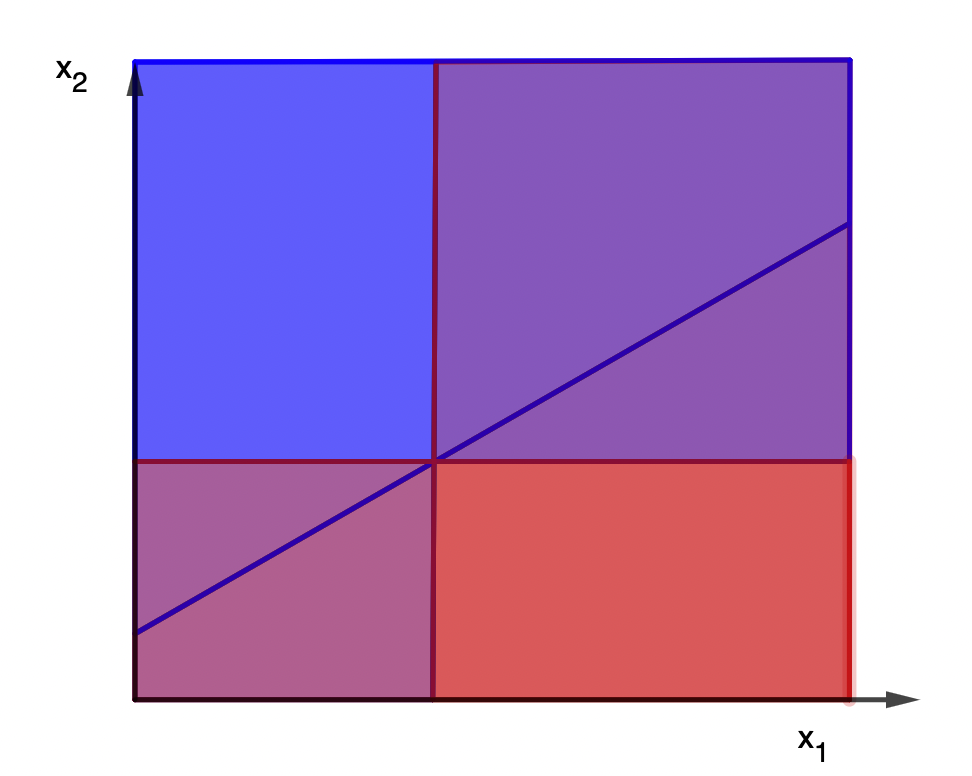
\includegraphics[width=0.65\linewidth]{../diagram_polariazation_2variables} 

}

\caption{\label{examp} Polarization regions for two single variable models}\label{fig:unnamed-chunk-1}
\end{figure}

For any pair of agents who observe the same realization of the
observables and use different models, it is possible to determine
whether they will be polarized or not by looking at the predictions made
by the optimal rule corresponding to their models. Polarizing
observations---those for which the predictions are different---are
different for each pair of models. Also notice that we determine whether
an observation is polarizing or not by using the optimal rules. We do
not expect subjects in our experiment to converge to the optimal rule,
this is a theoretical construct that allows us to formalize Prediction
2.

\textbf{Prediction 2 :} Polarization will arise more often when the
theory predicts so. That is, when two agents who have different models
of the world, are facing a realization of observables that polarizing
for their models.

\hypertarget{experimental-design}{%
\section{Experimental Design}\label{experimental-design}}

Subjects for the experimet were recruited from NYU's CESS-lab subject
pool. We recruited 30 undergraduate students who participated in this
experiment in person during the summer and fall of 2023. The experiment
was coded using oTree (\citet{otree}) and it consisted of two parts:
Part 1 was meant to expose the subjects to the data generating process
and allow them to learn how to predict the state; part 2 was meant to
elicit the models of the world that subjects might have developed in
part 1.

Part 1 consited of 20 rounds in which subjects observed the realizations
of all of the observables and were asked to predict the state. We had 5
observable variables called variable 1, 2, 3, 4 and 5. The variables
were independent and Normally distributed with means and variances as
described in Table \ref{params}.

The state was determined by the following linear rule:
\(11x_1+6x_2+4.5x_3+2.4x_4+k \geq 0\). The values of the coefficients
were chosen so that all variables had a similar but unique level of
informativeness when considered on their own. The constant \(k\) was
chosen so that the state was \textbf{B} in 50\% of the cases. The last
column of Table \ref{params} shows the probability of the optimal
prediction rule making a correct prediction when for each
single-variable model. This is the measure that we use to determine the
informativeness of each variable.

\begin{longtable}[]{@{}
  >{\raggedright\arraybackslash}p{(\columnwidth - 10\tabcolsep) * \real{0.1159}}
  >{\raggedright\arraybackslash}p{(\columnwidth - 10\tabcolsep) * \real{0.0580}}
  >{\raggedright\arraybackslash}p{(\columnwidth - 10\tabcolsep) * \real{0.1159}}
  >{\raggedright\arraybackslash}p{(\columnwidth - 10\tabcolsep) * \real{0.2464}}
  >{\raggedright\arraybackslash}p{(\columnwidth - 10\tabcolsep) * \real{0.2464}}
  >{\raggedright\arraybackslash}p{(\columnwidth - 10\tabcolsep) * \real{0.2174}}@{}}
\caption{Parameters for the Data Generating Process
\label{params}}\tabularnewline
\toprule\noalign{}
\begin{minipage}[b]{\linewidth}\raggedright
Variable
\end{minipage} & \begin{minipage}[b]{\linewidth}\raggedright
Mean
\end{minipage} & \begin{minipage}[b]{\linewidth}\raggedright
Variance
\end{minipage} & \begin{minipage}[b]{\linewidth}\raggedright
Modified Variable
\end{minipage} & \begin{minipage}[b]{\linewidth}\raggedright
Modified Variance
\end{minipage} & \begin{minipage}[b]{\linewidth}\raggedright
Informativeness
\end{minipage} \\
\midrule\noalign{}
\endfirsthead
\toprule\noalign{}
\begin{minipage}[b]{\linewidth}\raggedright
Variable
\end{minipage} & \begin{minipage}[b]{\linewidth}\raggedright
Mean
\end{minipage} & \begin{minipage}[b]{\linewidth}\raggedright
Variance
\end{minipage} & \begin{minipage}[b]{\linewidth}\raggedright
Modified Variable
\end{minipage} & \begin{minipage}[b]{\linewidth}\raggedright
Modified Variance
\end{minipage} & \begin{minipage}[b]{\linewidth}\raggedright
Informativeness
\end{minipage} \\
\midrule\noalign{}
\endhead
\bottomrule\noalign{}
\endlastfoot
\(x_1\) & 0 & 1 & \(11x_1\) & 11 & .65 \\
\(x_2\) & -10 & 2 & \(6x_2\) & 12 & .67 \\
\(x_3\) & 5 & 3 & \(4.5x_3\) & 13.5 & .69 \\
\(x_4\) & -5 & 4 & \(2.4*x_4\) & 12 & .63 \\
\(x_5\) & 100 & 5 & \(0x_5\) & 0 & 0 \\
\end{longtable}

In each round, subjects were asked to predict the state. They were given
feedback on whether their prediction was correct or not and they had
access to the entire history of the game. Throughout the experiment,
subjects were paired with another participant at random. Both subjects
in a pair were shown exactly the same realization of the variables and
had to predict the same state. This allows us to determine whether the
pair was polarized for that particular observation. Subjects were not
told that there was someone else observing the same realizations as
them.

Part 2 started immediatly after part 1 and had 70
rounds\footnote{In the first 2 sessions we had 40 rounds in part 2
and the experiment was done in under 30 minutes. Because the experiment concluded in less time than expected, we increased the 
number of rounds to 70 for the following sessions. Only 12 of our subjects participated in the sessions with 40 rounds, all others 
were in sessions with 70 rounds for part 2}. In instead of showing
subjects the realizations of all 5 variables, they were told that they
can disclose up to \(m\) variables, where \(m\) was drawn at random from
the set \(\{1, 2, ..., 5\}\). m was redrawn independently across rounds
and across subjects.

We use the random assignment of \(m\) to investigate whether the
subjects are using siumple or complex models. If allowing subjects to
disclose an additional variable improves their prediction accuracy, then
it must be that they are in fact using the additional information for
prediciton. If, on the other hand, they do not perform better when they
have access to more information, it must be that, although they are
disclosing an additional variable, they do not correctly incorporate the
infomation into their prediction rule. Thus, if we observe that the
performance of our subjects does not improve when they are allowed to
disclose \(m+1\) variables, relative to their performance when they were
allowed to disclose only \(m\) variables, their model of the world must
be of size \(m\) or lower. This feature design allows us to test
predictions 1 and 1B and determine the number of variables that subjects
are using.

In order to explore the polarization prediction, we use the fact that
subjects are in fixed pairs throughout the experiment. Both subjects in
a pair observe the same realization of all the variables in each round.
Therefore, we can determine whether they are polarized or not by looking
at whether they make the same prediction or not. We can then determine
whether the theory predicts that they should be polarized or not by
looking at what the optimal rules for those models dictate. We use the
optimal rules that correcpond to the variables that they chose to reveal
in that round. It could be that although they are revealing certain
variables, they are not using them for prediction. Since we do not have
a good method to determine which variables they actually pay attention
to, we use the variables that they reveal as a proxy for the variables
that they are using for prediction and apply the optimal rules for those
models.

\hypertarget{results}{%
\section{Results}\label{results}}

In this section we present the results from the experiment. We start by
exploring the general learning patterns of the subjects as well as the
model choices. We then look at the effect of allowing subjects to
disclose an additional variable and lastly we look at the polarization
results.

\subsection{Learning}

In the first part of the experiment, subjects were asked to predict the
state given the realization of all the variables. Having access to all
the information they could predict the state perfectly if they managed
to learn the parameters of the hyperplane that determines the state.
Figure \ref{learningAll} shows the share of correct predictions across
rounds in part 1. We see that subjects are able to learn how to predict
the state at a rate that is higher than random. They initially predict
the state corectly about 50\% of the time, which is consistent with
random guessing. The share of correct guesses increases to 59\% by the
end of part 1. And this last number is significantly higher than 50\%
(p-value = 0.00031). They continue to learn even after the first 20
rounds when we look at the rounds in which subjects had access to all
the information. By the end of the experiment the rate of correct
predictions is 59\% which is still significantly higher than 50\%
(p-value = 0.00000019).

\begin{figure}

{\centering 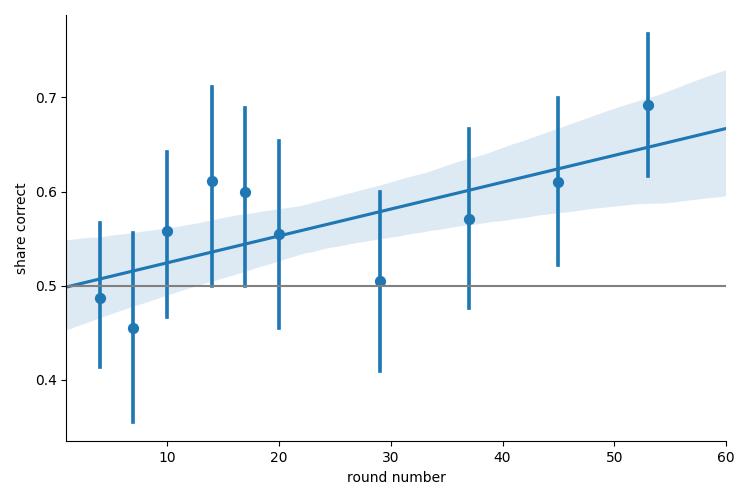
\includegraphics[width=0.65\linewidth]{../computed_objects/figures/learning_all} 

}

\caption{\label{learningAll} Share of correct predictions across rounds by performance in rounds 20 to 40}\label{fig:learningAll}
\end{figure}

We also observe that there is heterogeneity in how our subjects learn.
In particular, in the first 20 rounds of part 2 we are able to identify
two distinct groups of subjects: those who guess more than 50\% of the
states correctly and those who guess 50\% of fewer of them correctly. As
can seen in \ref{p2groups}, these two groups have very different
learning patterns throughout the experiment. The group that does better
than random in rounds 20 to 40 (the first 20 rounds of part 2) consists
of 20 subjects, which account for 67\% of the sample. These subjects
improved their performance from 50\% to 64\% in the first 20 rounds of
part 2, and continued to improve to get to 69\% by the end of part 2.
Meanwhile, the group that does worse than random in rounds 20 to 40
consists of 10 subjects and they do not seem to learn how to predict the
state more accurately even after all 60 rounds of the experiment.
Whenever it is relevant, we will show results separately for these two
groups.

\begin{figure}

{\centering 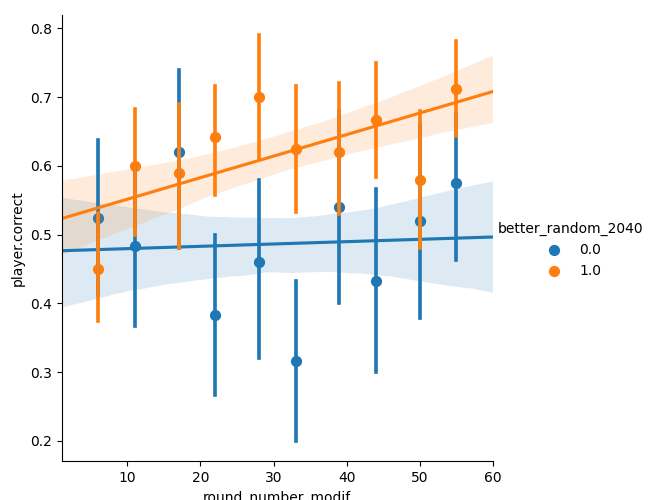
\includegraphics[width=0.65\linewidth]{../computed_objects/figures/p2_correct_rounds} 

}

\caption{\label{p2groups} Share of correct predictions across rounds}\label{fig:p2groups}
\end{figure}

\hypertarget{simplicity}{%
\subsection{Simplicity}\label{simplicity}}

In part 2, subjects were allowed to disclose up to \(m\) variables
before making their predictions. and \(m\) was assigned at random for
every subject in every round. We use this random assignment to
understand if allowing them to reveal an additional variable improves
their prediction accuracy. If it does, it must be that they are using
the additional information for prediction. Figure \ref{simplicity} shows
the share of correct predictions by the number of variables that
subjects chose to disclose. Figure \ref{simplicity2} shows the number of
variables that subjects chose to disclose by the number they we allowed
to disclose. On average, they always disclose fewer variables than what
is available to them. This is a strong indication that at least some of
the subjects are using simple models. Further evidence is provided by
the accuracy of their predictions as discussed in what follows

\begin{figure}

{\centering 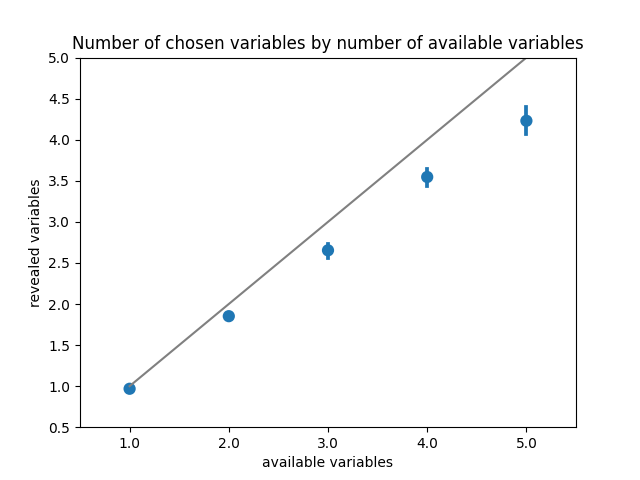
\includegraphics[width=0.65\linewidth]{../computed_objects/figures/revealed_available} 

}

\caption{\label{simplicity2} Number of disclosed variables by number of allowed variables}\label{fig:simplicity2}
\end{figure}

\begin{figure}

{\centering 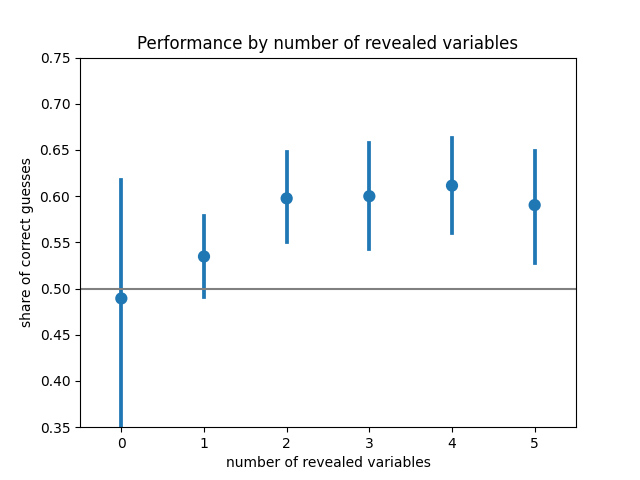
\includegraphics[width=0.65\linewidth]{../computed_objects/figures/revealed_variables_pooled} 

}

\caption{\label{simplicity} Share of correct predictions by number of disclosed variables}\label{fig:simplicity}
\end{figure}

We see that there is a sharp increase when going from 1 to 2 variables,
but no significant increase when going from 2 to 3 and beyond. This
suggests that on average subjects are using mental models that consider
2 variables. However, since subjects were allowed to reveal fewer
variables than what was assigned to them, the estimates in
\ref{simplicity} might be biased. To account for this, we also look at
the share of correct predictions by the number of variables that
subjects were allowed to disclose. The results are presented in Table
\ref{regression_table}. The table presents the regression estimates for
the model with the assigned number of variables as well as the model
with the number of variables that subjects chose to disclose. The last
column clusters standard errors at the group level.

 
  \providecommand{\huxb}[2]{\arrayrulecolor[RGB]{#1}\global\arrayrulewidth=#2pt}
  \providecommand{\huxvb}[2]{\color[RGB]{#1}\vrule width #2pt}
  \providecommand{\huxtpad}[1]{\rule{0pt}{#1}}
  \providecommand{\huxbpad}[1]{\rule[-#1]{0pt}{#1}}

\begin{table}[ht]
\begin{centerbox}
\begin{threeparttable}
\captionsetup{justification=centering,singlelinecheck=off}
\caption{Regression results, dependent variable is the share of correct predictions.}
 \label{regression_table}
\setlength{\tabcolsep}{0pt}
\begin{tabular}{l l l l}


\hhline{>{\huxb{0, 0, 0}{0.8}}->{\huxb{0, 0, 0}{0.8}}->{\huxb{0, 0, 0}{0.8}}->{\huxb{0, 0, 0}{0.8}}-}
\arrayrulecolor{black}

\multicolumn{1}{!{\huxvb{0, 0, 0}{0}}c!{\huxvb{0, 0, 0}{0}}}{\huxtpad{6pt + 1em}\centering \hspace{6pt}  \hspace{6pt}\huxbpad{6pt}} &
\multicolumn{1}{c!{\huxvb{0, 0, 0}{0}}}{\huxtpad{6pt + 1em}\centering \hspace{6pt} Disclosed \hspace{6pt}\huxbpad{6pt}} &
\multicolumn{1}{c!{\huxvb{0, 0, 0}{0}}}{\huxtpad{6pt + 1em}\centering \hspace{6pt} Allowed \hspace{6pt}\huxbpad{6pt}} &
\multicolumn{1}{c!{\huxvb{0, 0, 0}{0}}}{\huxtpad{6pt + 1em}\centering \hspace{6pt} Allowed \hspace{6pt}\huxbpad{6pt}} \tabularnewline[-0.5pt]


\hhline{>{\huxb{255, 255, 255}{0.4}}->{\huxb{0, 0, 0}{0.4}}->{\huxb{0, 0, 0}{0.4}}->{\huxb{0, 0, 0}{0.4}}-}
\arrayrulecolor{black}

\multicolumn{1}{!{\huxvb{0, 0, 0}{0}}l!{\huxvb{0, 0, 0}{0}}}{\huxtpad{6pt + 1em}\raggedright \hspace{6pt} Zero variables \hspace{6pt}\huxbpad{6pt}} &
\multicolumn{1}{r!{\huxvb{0, 0, 0}{0}}}{\huxtpad{6pt + 1em}\raggedleft \hspace{6pt} 0.489 *** \hspace{6pt}\huxbpad{6pt}} &
\multicolumn{1}{r!{\huxvb{0, 0, 0}{0}}}{\huxtpad{6pt + 1em}\raggedleft \hspace{6pt} \hphantom{0}\hphantom{0}\hphantom{0}\hphantom{0}\hphantom{0}\hphantom{0}\hphantom{0}\hphantom{0} \hspace{6pt}\huxbpad{6pt}} &
\multicolumn{1}{r!{\huxvb{0, 0, 0}{0}}}{\huxtpad{6pt + 1em}\raggedleft \hspace{6pt} \hphantom{0}\hphantom{0}\hphantom{0}\hphantom{0}\hphantom{0}\hphantom{0}\hphantom{0}\hphantom{0} \hspace{6pt}\huxbpad{6pt}} \tabularnewline[-0.5pt]


\hhline{}
\arrayrulecolor{black}

\multicolumn{1}{!{\huxvb{0, 0, 0}{0}}l!{\huxvb{0, 0, 0}{0}}}{\huxtpad{6pt + 1em}\raggedright \hspace{6pt}  \hspace{6pt}\huxbpad{6pt}} &
\multicolumn{1}{r!{\huxvb{0, 0, 0}{0}}}{\huxtpad{6pt + 1em}\raggedleft \hspace{6pt} (0.072)\hphantom{0}\hphantom{0}\hphantom{0} \hspace{6pt}\huxbpad{6pt}} &
\multicolumn{1}{r!{\huxvb{0, 0, 0}{0}}}{\huxtpad{6pt + 1em}\raggedleft \hspace{6pt} \hphantom{0}\hphantom{0}\hphantom{0}\hphantom{0}\hphantom{0}\hphantom{0}\hphantom{0}\hphantom{0} \hspace{6pt}\huxbpad{6pt}} &
\multicolumn{1}{r!{\huxvb{0, 0, 0}{0}}}{\huxtpad{6pt + 1em}\raggedleft \hspace{6pt} \hphantom{0}\hphantom{0}\hphantom{0}\hphantom{0}\hphantom{0}\hphantom{0}\hphantom{0}\hphantom{0} \hspace{6pt}\huxbpad{6pt}} \tabularnewline[-0.5pt]


\hhline{}
\arrayrulecolor{black}

\multicolumn{1}{!{\huxvb{0, 0, 0}{0}}l!{\huxvb{0, 0, 0}{0}}}{\huxtpad{6pt + 1em}\raggedright \hspace{6pt} One variable \hspace{6pt}\huxbpad{6pt}} &
\multicolumn{1}{r!{\huxvb{0, 0, 0}{0}}}{\huxtpad{6pt + 1em}\raggedleft \hspace{6pt} 0.535 *** \hspace{6pt}\huxbpad{6pt}} &
\multicolumn{1}{r!{\huxvb{0, 0, 0}{0}}}{\huxtpad{6pt + 1em}\raggedleft \hspace{6pt} 0.534 *** \hspace{6pt}\huxbpad{6pt}} &
\multicolumn{1}{r!{\huxvb{0, 0, 0}{0}}}{\huxtpad{6pt + 1em}\raggedleft \hspace{6pt} 0.534 *** \hspace{6pt}\huxbpad{6pt}} \tabularnewline[-0.5pt]


\hhline{}
\arrayrulecolor{black}

\multicolumn{1}{!{\huxvb{0, 0, 0}{0}}l!{\huxvb{0, 0, 0}{0}}}{\huxtpad{6pt + 1em}\raggedright \hspace{6pt}  \hspace{6pt}\huxbpad{6pt}} &
\multicolumn{1}{r!{\huxvb{0, 0, 0}{0}}}{\huxtpad{6pt + 1em}\raggedleft \hspace{6pt} (0.023)\hphantom{0}\hphantom{0}\hphantom{0} \hspace{6pt}\huxbpad{6pt}} &
\multicolumn{1}{r!{\huxvb{0, 0, 0}{0}}}{\huxtpad{6pt + 1em}\raggedleft \hspace{6pt} (0.027)\hphantom{0}\hphantom{0}\hphantom{0} \hspace{6pt}\huxbpad{6pt}} &
\multicolumn{1}{r!{\huxvb{0, 0, 0}{0}}}{\huxtpad{6pt + 1em}\raggedleft \hspace{6pt} (0.033)\hphantom{0}\hphantom{0}\hphantom{0} \hspace{6pt}\huxbpad{6pt}} \tabularnewline[-0.5pt]


\hhline{}
\arrayrulecolor{black}

\multicolumn{1}{!{\huxvb{0, 0, 0}{0}}l!{\huxvb{0, 0, 0}{0}}}{\huxtpad{6pt + 1em}\raggedright \hspace{6pt} Two variables \hspace{6pt}\huxbpad{6pt}} &
\multicolumn{1}{r!{\huxvb{0, 0, 0}{0}}}{\huxtpad{6pt + 1em}\raggedleft \hspace{6pt} 0.598 *** \hspace{6pt}\huxbpad{6pt}} &
\multicolumn{1}{r!{\huxvb{0, 0, 0}{0}}}{\huxtpad{6pt + 1em}\raggedleft \hspace{6pt} 0.602 *** \hspace{6pt}\huxbpad{6pt}} &
\multicolumn{1}{r!{\huxvb{0, 0, 0}{0}}}{\huxtpad{6pt + 1em}\raggedleft \hspace{6pt} 0.602 *** \hspace{6pt}\huxbpad{6pt}} \tabularnewline[-0.5pt]


\hhline{}
\arrayrulecolor{black}

\multicolumn{1}{!{\huxvb{0, 0, 0}{0}}l!{\huxvb{0, 0, 0}{0}}}{\huxtpad{6pt + 1em}\raggedright \hspace{6pt}  \hspace{6pt}\huxbpad{6pt}} &
\multicolumn{1}{r!{\huxvb{0, 0, 0}{0}}}{\huxtpad{6pt + 1em}\raggedleft \hspace{6pt} (0.027)\hphantom{0}\hphantom{0}\hphantom{0} \hspace{6pt}\huxbpad{6pt}} &
\multicolumn{1}{r!{\huxvb{0, 0, 0}{0}}}{\huxtpad{6pt + 1em}\raggedleft \hspace{6pt} (0.027)\hphantom{0}\hphantom{0}\hphantom{0} \hspace{6pt}\huxbpad{6pt}} &
\multicolumn{1}{r!{\huxvb{0, 0, 0}{0}}}{\huxtpad{6pt + 1em}\raggedleft \hspace{6pt} (0.028)\hphantom{0}\hphantom{0}\hphantom{0} \hspace{6pt}\huxbpad{6pt}} \tabularnewline[-0.5pt]


\hhline{}
\arrayrulecolor{black}

\multicolumn{1}{!{\huxvb{0, 0, 0}{0}}l!{\huxvb{0, 0, 0}{0}}}{\huxtpad{6pt + 1em}\raggedright \hspace{6pt} Three variables \hspace{6pt}\huxbpad{6pt}} &
\multicolumn{1}{r!{\huxvb{0, 0, 0}{0}}}{\huxtpad{6pt + 1em}\raggedleft \hspace{6pt} 0.600 *** \hspace{6pt}\huxbpad{6pt}} &
\multicolumn{1}{r!{\huxvb{0, 0, 0}{0}}}{\huxtpad{6pt + 1em}\raggedleft \hspace{6pt} 0.584 *** \hspace{6pt}\huxbpad{6pt}} &
\multicolumn{1}{r!{\huxvb{0, 0, 0}{0}}}{\huxtpad{6pt + 1em}\raggedleft \hspace{6pt} 0.584 *** \hspace{6pt}\huxbpad{6pt}} \tabularnewline[-0.5pt]


\hhline{}
\arrayrulecolor{black}

\multicolumn{1}{!{\huxvb{0, 0, 0}{0}}l!{\huxvb{0, 0, 0}{0}}}{\huxtpad{6pt + 1em}\raggedright \hspace{6pt}  \hspace{6pt}\huxbpad{6pt}} &
\multicolumn{1}{r!{\huxvb{0, 0, 0}{0}}}{\huxtpad{6pt + 1em}\raggedleft \hspace{6pt} (0.029)\hphantom{0}\hphantom{0}\hphantom{0} \hspace{6pt}\huxbpad{6pt}} &
\multicolumn{1}{r!{\huxvb{0, 0, 0}{0}}}{\huxtpad{6pt + 1em}\raggedleft \hspace{6pt} (0.027)\hphantom{0}\hphantom{0}\hphantom{0} \hspace{6pt}\huxbpad{6pt}} &
\multicolumn{1}{r!{\huxvb{0, 0, 0}{0}}}{\huxtpad{6pt + 1em}\raggedleft \hspace{6pt} (0.031)\hphantom{0}\hphantom{0}\hphantom{0} \hspace{6pt}\huxbpad{6pt}} \tabularnewline[-0.5pt]


\hhline{}
\arrayrulecolor{black}

\multicolumn{1}{!{\huxvb{0, 0, 0}{0}}l!{\huxvb{0, 0, 0}{0}}}{\huxtpad{6pt + 1em}\raggedright \hspace{6pt} Four variables \hspace{6pt}\huxbpad{6pt}} &
\multicolumn{1}{r!{\huxvb{0, 0, 0}{0}}}{\huxtpad{6pt + 1em}\raggedleft \hspace{6pt} 0.611 *** \hspace{6pt}\huxbpad{6pt}} &
\multicolumn{1}{r!{\huxvb{0, 0, 0}{0}}}{\huxtpad{6pt + 1em}\raggedleft \hspace{6pt} 0.599 *** \hspace{6pt}\huxbpad{6pt}} &
\multicolumn{1}{r!{\huxvb{0, 0, 0}{0}}}{\huxtpad{6pt + 1em}\raggedleft \hspace{6pt} 0.599 *** \hspace{6pt}\huxbpad{6pt}} \tabularnewline[-0.5pt]


\hhline{}
\arrayrulecolor{black}

\multicolumn{1}{!{\huxvb{0, 0, 0}{0}}l!{\huxvb{0, 0, 0}{0}}}{\huxtpad{6pt + 1em}\raggedright \hspace{6pt}  \hspace{6pt}\huxbpad{6pt}} &
\multicolumn{1}{r!{\huxvb{0, 0, 0}{0}}}{\huxtpad{6pt + 1em}\raggedleft \hspace{6pt} (0.028)\hphantom{0}\hphantom{0}\hphantom{0} \hspace{6pt}\huxbpad{6pt}} &
\multicolumn{1}{r!{\huxvb{0, 0, 0}{0}}}{\huxtpad{6pt + 1em}\raggedleft \hspace{6pt} (0.025)\hphantom{0}\hphantom{0}\hphantom{0} \hspace{6pt}\huxbpad{6pt}} &
\multicolumn{1}{r!{\huxvb{0, 0, 0}{0}}}{\huxtpad{6pt + 1em}\raggedleft \hspace{6pt} (0.042)\hphantom{0}\hphantom{0}\hphantom{0} \hspace{6pt}\huxbpad{6pt}} \tabularnewline[-0.5pt]


\hhline{}
\arrayrulecolor{black}

\multicolumn{1}{!{\huxvb{0, 0, 0}{0}}l!{\huxvb{0, 0, 0}{0}}}{\huxtpad{6pt + 1em}\raggedright \hspace{6pt} Five variables \hspace{6pt}\huxbpad{6pt}} &
\multicolumn{1}{r!{\huxvb{0, 0, 0}{0}}}{\huxtpad{6pt + 1em}\raggedleft \hspace{6pt} 0.590 *** \hspace{6pt}\huxbpad{6pt}} &
\multicolumn{1}{r!{\huxvb{0, 0, 0}{0}}}{\huxtpad{6pt + 1em}\raggedleft \hspace{6pt} 0.576 *** \hspace{6pt}\huxbpad{6pt}} &
\multicolumn{1}{r!{\huxvb{0, 0, 0}{0}}}{\huxtpad{6pt + 1em}\raggedleft \hspace{6pt} 0.576 *** \hspace{6pt}\huxbpad{6pt}} \tabularnewline[-0.5pt]


\hhline{}
\arrayrulecolor{black}

\multicolumn{1}{!{\huxvb{0, 0, 0}{0}}l!{\huxvb{0, 0, 0}{0}}}{\huxtpad{6pt + 1em}\raggedright \hspace{6pt}  \hspace{6pt}\huxbpad{6pt}} &
\multicolumn{1}{r!{\huxvb{0, 0, 0}{0}}}{\huxtpad{6pt + 1em}\raggedleft \hspace{6pt} (0.030)\hphantom{0}\hphantom{0}\hphantom{0} \hspace{6pt}\huxbpad{6pt}} &
\multicolumn{1}{r!{\huxvb{0, 0, 0}{0}}}{\huxtpad{6pt + 1em}\raggedleft \hspace{6pt} (0.027)\hphantom{0}\hphantom{0}\hphantom{0} \hspace{6pt}\huxbpad{6pt}} &
\multicolumn{1}{r!{\huxvb{0, 0, 0}{0}}}{\huxtpad{6pt + 1em}\raggedleft \hspace{6pt} (0.040)\hphantom{0}\hphantom{0}\hphantom{0} \hspace{6pt}\huxbpad{6pt}} \tabularnewline[-0.5pt]


\hhline{>{\huxb{255, 255, 255}{0.4}}->{\huxb{0, 0, 0}{0.4}}->{\huxb{0, 0, 0}{0.4}}->{\huxb{0, 0, 0}{0.4}}-}
\arrayrulecolor{black}

\multicolumn{1}{!{\huxvb{0, 0, 0}{0}}l!{\huxvb{0, 0, 0}{0}}}{\huxtpad{6pt + 1em}\raggedright \hspace{6pt} Clustered SE \hspace{6pt}\huxbpad{6pt}} &
\multicolumn{1}{r!{\huxvb{0, 0, 0}{0}}}{\huxtpad{6pt + 1em}\raggedleft \hspace{6pt} NO\hphantom{0}\hphantom{0}\hphantom{0}\hphantom{0}\hphantom{0}\hphantom{0}\hphantom{0}\hphantom{0} \hspace{6pt}\huxbpad{6pt}} &
\multicolumn{1}{r!{\huxvb{0, 0, 0}{0}}}{\huxtpad{6pt + 1em}\raggedleft \hspace{6pt} NO\hphantom{0}\hphantom{0}\hphantom{0}\hphantom{0}\hphantom{0}\hphantom{0}\hphantom{0}\hphantom{0} \hspace{6pt}\huxbpad{6pt}} &
\multicolumn{1}{r!{\huxvb{0, 0, 0}{0}}}{\huxtpad{6pt + 1em}\raggedleft \hspace{6pt} Group\hphantom{0}\hphantom{0}\hphantom{0}\hphantom{0}\hphantom{0}\hphantom{0}\hphantom{0}\hphantom{0} \hspace{6pt}\huxbpad{6pt}} \tabularnewline[-0.5pt]


\hhline{>{\huxb{255, 255, 255}{0.4}}->{\huxb{0, 0, 0}{0.4}}->{\huxb{0, 0, 0}{0.4}}->{\huxb{0, 0, 0}{0.4}}-}
\arrayrulecolor{black}

\multicolumn{1}{!{\huxvb{0, 0, 0}{0}}l!{\huxvb{0, 0, 0}{0}}}{\huxtpad{6pt + 1em}\raggedright \hspace{6pt} N. obs. \hspace{6pt}\huxbpad{6pt}} &
\multicolumn{1}{r!{\huxvb{0, 0, 0}{0}}}{\huxtpad{6pt + 1em}\raggedleft \hspace{6pt} 1740\hphantom{0}\hphantom{0}\hphantom{0}\hphantom{0}\hphantom{0}\hphantom{0}\hphantom{0}\hphantom{0} \hspace{6pt}\huxbpad{6pt}} &
\multicolumn{1}{r!{\huxvb{0, 0, 0}{0}}}{\huxtpad{6pt + 1em}\raggedleft \hspace{6pt} 1740\hphantom{0}\hphantom{0}\hphantom{0}\hphantom{0}\hphantom{0}\hphantom{0}\hphantom{0}\hphantom{0} \hspace{6pt}\huxbpad{6pt}} &
\multicolumn{1}{r!{\huxvb{0, 0, 0}{0}}}{\huxtpad{6pt + 1em}\raggedleft \hspace{6pt} 1740\hphantom{0}\hphantom{0}\hphantom{0}\hphantom{0}\hphantom{0}\hphantom{0}\hphantom{0}\hphantom{0} \hspace{6pt}\huxbpad{6pt}} \tabularnewline[-0.5pt]


\hhline{}
\arrayrulecolor{black}

\multicolumn{1}{!{\huxvb{0, 0, 0}{0}}l!{\huxvb{0, 0, 0}{0}}}{\huxtpad{6pt + 1em}\raggedright \hspace{6pt} R squared \hspace{6pt}\huxbpad{6pt}} &
\multicolumn{1}{r!{\huxvb{0, 0, 0}{0}}}{\huxtpad{6pt + 1em}\raggedleft \hspace{6pt} 0.581\hphantom{0}\hphantom{0}\hphantom{0}\hphantom{0} \hspace{6pt}\huxbpad{6pt}} &
\multicolumn{1}{r!{\huxvb{0, 0, 0}{0}}}{\huxtpad{6pt + 1em}\raggedleft \hspace{6pt} 0.580\hphantom{0}\hphantom{0}\hphantom{0}\hphantom{0} \hspace{6pt}\huxbpad{6pt}} &
\multicolumn{1}{r!{\huxvb{0, 0, 0}{0}}}{\huxtpad{6pt + 1em}\raggedleft \hspace{6pt} 0.580\hphantom{0}\hphantom{0}\hphantom{0}\hphantom{0} \hspace{6pt}\huxbpad{6pt}} \tabularnewline[-0.5pt]


\hhline{>{\huxb{0, 0, 0}{0.8}}->{\huxb{0, 0, 0}{0.8}}->{\huxb{0, 0, 0}{0.8}}->{\huxb{0, 0, 0}{0.8}}-}
\arrayrulecolor{black}

\multicolumn{4}{!{\huxvb{0, 0, 0}{0}}l!{\huxvb{0, 0, 0}{0}}}{\huxtpad{6pt + 1em}\raggedright \hspace{6pt}  *** p $<$ 0.001;  ** p $<$ 0.01;  * p $<$ 0.05. \hspace{6pt}\huxbpad{6pt}} \tabularnewline[-0.5pt]


\hhline{}
\arrayrulecolor{black}
\end{tabular}
\end{threeparttable}\par\end{centerbox}

\end{table}
 

We are interested in testing whether the probability of guessing the
state correctly increases when subjects are allowed to disclose an
additional variable. This corresponds to testing the linear hypotheses
\(\beta_{m+1}-\beta_m=0\) for \(m=1, 2, 3, 4\). The results of these
tests are presented in Table \ref{hypotheses}. We see that the
probability of guessing the state when subjects are allowed to disclose
2 variables is significantly higher than when they are allowed to
disclose only 1 variable. And the effect of having access to the
additional variable is 0.068 percentage points. Allowing 3, 4 and 5
variables has no effect, which sugests that subjects are using models
that consider 2 variables. All the hypothesis tests are reported in
Tables \ref{test_assigned},\ref{test_revealed} and \ref{test_clustered}
in the appendix.

\hypertarget{model-choices}{%
\subsection{Model Choices}\label{model-choices}}

Since we now know that subjects are using models that consider 2
variables, we can look at the specific models that they are using. We
look at two particular features: Are they choosing the most informative
models? and do they improve their model choices over time?

\hypertarget{polarization-results}{%
\subsection{Polarization Results}\label{polarization-results}}

\hypertarget{conclusion}{%
\section{Conclusion}\label{conclusion}}

\newpage
\appendix

\hypertarget{appendix}{%
\section{Appendix}\label{appendix}}

 
  \providecommand{\huxb}[2]{\arrayrulecolor[RGB]{#1}\global\arrayrulewidth=#2pt}
  \providecommand{\huxvb}[2]{\color[RGB]{#1}\vrule width #2pt}
  \providecommand{\huxtpad}[1]{\rule{0pt}{#1}}
  \providecommand{\huxbpad}[1]{\rule[-#1]{0pt}{#1}}

\begin{table}[ht]
\begin{centerbox}
\begin{threeparttable}
\captionsetup{justification=centering,singlelinecheck=off}
\caption{Hypothesis tests for the regression with the number of variables that subjects chose to disclose.}
 \label{test_revealed}
\setlength{\tabcolsep}{0pt}
\begin{tabular}{l l l}


\hhline{}
\arrayrulecolor{black}

\multicolumn{1}{!{\huxvb{0, 0, 0}{0}}l!{\huxvb{0, 0, 0}{0}}}{\huxtpad{6pt + 1em}\raggedright \hspace{6pt} Hypothesis \hspace{6pt}\huxbpad{6pt}} &
\multicolumn{1}{r!{\huxvb{0, 0, 0}{0}}}{\huxtpad{6pt + 1em}\raggedleft \hspace{6pt} Estimate \hspace{6pt}\huxbpad{6pt}} &
\multicolumn{1}{r!{\huxvb{0, 0, 0}{0}}}{\huxtpad{6pt + 1em}\raggedleft \hspace{6pt} p-value \hspace{6pt}\huxbpad{6pt}} \tabularnewline[-0.5pt]


\hhline{}
\arrayrulecolor{black}

\multicolumn{1}{!{\huxvb{0, 0, 0}{0}}l!{\huxvb{0, 0, 0}{0}}}{\huxtpad{6pt + 1em}\raggedright \hspace{6pt} b\_0=.5 \hspace{6pt}\huxbpad{6pt}} &
\multicolumn{1}{r!{\huxvb{0, 0, 0}{0}}}{\huxtpad{6pt + 1em}\raggedleft \hspace{6pt} -0.0106\hphantom{0} \hspace{6pt}\huxbpad{6pt}} &
\multicolumn{1}{r!{\huxvb{0, 0, 0}{0}}}{\huxtpad{6pt + 1em}\raggedleft \hspace{6pt} 0.883\hphantom{0} \hspace{6pt}\huxbpad{6pt}} \tabularnewline[-0.5pt]


\hhline{}
\arrayrulecolor{black}

\multicolumn{1}{!{\huxvb{0, 0, 0}{0}}l!{\huxvb{0, 0, 0}{0}}}{\huxtpad{6pt + 1em}\raggedright \hspace{6pt} b\_1-b0=0 \hspace{6pt}\huxbpad{6pt}} &
\multicolumn{1}{r!{\huxvb{0, 0, 0}{0}}}{\huxtpad{6pt + 1em}\raggedleft \hspace{6pt} 0.0454\hphantom{0} \hspace{6pt}\huxbpad{6pt}} &
\multicolumn{1}{r!{\huxvb{0, 0, 0}{0}}}{\huxtpad{6pt + 1em}\raggedleft \hspace{6pt} 0.548\hphantom{0} \hspace{6pt}\huxbpad{6pt}} \tabularnewline[-0.5pt]


\hhline{}
\arrayrulecolor{black}

\multicolumn{1}{!{\huxvb{0, 0, 0}{0}}l!{\huxvb{0, 0, 0}{0}}}{\huxtpad{6pt + 1em}\raggedright \hspace{6pt} b\_2-b1=0 \hspace{6pt}\huxbpad{6pt}} &
\multicolumn{1}{r!{\huxvb{0, 0, 0}{0}}}{\huxtpad{6pt + 1em}\raggedleft \hspace{6pt} 0.0629\hphantom{0} \hspace{6pt}\huxbpad{6pt}} &
\multicolumn{1}{r!{\huxvb{0, 0, 0}{0}}}{\huxtpad{6pt + 1em}\raggedleft \hspace{6pt} 0.0734 \hspace{6pt}\huxbpad{6pt}} \tabularnewline[-0.5pt]


\hhline{}
\arrayrulecolor{black}

\multicolumn{1}{!{\huxvb{0, 0, 0}{0}}l!{\huxvb{0, 0, 0}{0}}}{\huxtpad{6pt + 1em}\raggedright \hspace{6pt} b\_3-b2=0 \hspace{6pt}\huxbpad{6pt}} &
\multicolumn{1}{r!{\huxvb{0, 0, 0}{0}}}{\huxtpad{6pt + 1em}\raggedleft \hspace{6pt} 0.00237 \hspace{6pt}\huxbpad{6pt}} &
\multicolumn{1}{r!{\huxvb{0, 0, 0}{0}}}{\huxtpad{6pt + 1em}\raggedleft \hspace{6pt} 0.952\hphantom{0} \hspace{6pt}\huxbpad{6pt}} \tabularnewline[-0.5pt]


\hhline{}
\arrayrulecolor{black}

\multicolumn{1}{!{\huxvb{0, 0, 0}{0}}l!{\huxvb{0, 0, 0}{0}}}{\huxtpad{6pt + 1em}\raggedright \hspace{6pt} b\_4-b3=0 \hspace{6pt}\huxbpad{6pt}} &
\multicolumn{1}{r!{\huxvb{0, 0, 0}{0}}}{\huxtpad{6pt + 1em}\raggedleft \hspace{6pt} 0.0115\hphantom{0} \hspace{6pt}\huxbpad{6pt}} &
\multicolumn{1}{r!{\huxvb{0, 0, 0}{0}}}{\huxtpad{6pt + 1em}\raggedleft \hspace{6pt} 0.774\hphantom{0} \hspace{6pt}\huxbpad{6pt}} \tabularnewline[-0.5pt]


\hhline{}
\arrayrulecolor{black}

\multicolumn{1}{!{\huxvb{0, 0, 0}{0}}l!{\huxvb{0, 0, 0}{0}}}{\huxtpad{6pt + 1em}\raggedright \hspace{6pt} b\_5-b4=0 \hspace{6pt}\huxbpad{6pt}} &
\multicolumn{1}{r!{\huxvb{0, 0, 0}{0}}}{\huxtpad{6pt + 1em}\raggedleft \hspace{6pt} -0.0211\hphantom{0} \hspace{6pt}\huxbpad{6pt}} &
\multicolumn{1}{r!{\huxvb{0, 0, 0}{0}}}{\huxtpad{6pt + 1em}\raggedleft \hspace{6pt} 0.607\hphantom{0} \hspace{6pt}\huxbpad{6pt}} \tabularnewline[-0.5pt]


\hhline{}
\arrayrulecolor{black}
\end{tabular}
\end{threeparttable}\par\end{centerbox}

\end{table}
 

 
  \providecommand{\huxb}[2]{\arrayrulecolor[RGB]{#1}\global\arrayrulewidth=#2pt}
  \providecommand{\huxvb}[2]{\color[RGB]{#1}\vrule width #2pt}
  \providecommand{\huxtpad}[1]{\rule{0pt}{#1}}
  \providecommand{\huxbpad}[1]{\rule[-#1]{0pt}{#1}}

\begin{table}[ht]
\begin{centerbox}
\begin{threeparttable}
\captionsetup{justification=centering,singlelinecheck=off}
\caption{Hypothesis tests for the regression with the number of variables that subjects were allowed to disclose.}
 \label{test_assigned}
\setlength{\tabcolsep}{0pt}
\begin{tabular}{l l l}


\hhline{}
\arrayrulecolor{black}

\multicolumn{1}{!{\huxvb{0, 0, 0}{0}}l!{\huxvb{0, 0, 0}{0}}}{\huxtpad{6pt + 1em}\raggedright \hspace{6pt} Hypothesis \hspace{6pt}\huxbpad{6pt}} &
\multicolumn{1}{r!{\huxvb{0, 0, 0}{0}}}{\huxtpad{6pt + 1em}\raggedleft \hspace{6pt} Estimate \hspace{6pt}\huxbpad{6pt}} &
\multicolumn{1}{r!{\huxvb{0, 0, 0}{0}}}{\huxtpad{6pt + 1em}\raggedleft \hspace{6pt} p-value \hspace{6pt}\huxbpad{6pt}} \tabularnewline[-0.5pt]


\hhline{}
\arrayrulecolor{black}

\multicolumn{1}{!{\huxvb{0, 0, 0}{0}}l!{\huxvb{0, 0, 0}{0}}}{\huxtpad{6pt + 1em}\raggedright \hspace{6pt} b\_1=.5 \hspace{6pt}\huxbpad{6pt}} &
\multicolumn{1}{r!{\huxvb{0, 0, 0}{0}}}{\huxtpad{6pt + 1em}\raggedleft \hspace{6pt} 0.0335 \hspace{6pt}\huxbpad{6pt}} &
\multicolumn{1}{r!{\huxvb{0, 0, 0}{0}}}{\huxtpad{6pt + 1em}\raggedleft \hspace{6pt} 0.209\hphantom{0} \hspace{6pt}\huxbpad{6pt}} \tabularnewline[-0.5pt]


\hhline{}
\arrayrulecolor{black}

\multicolumn{1}{!{\huxvb{0, 0, 0}{0}}l!{\huxvb{0, 0, 0}{0}}}{\huxtpad{6pt + 1em}\raggedright \hspace{6pt} b\_2-b1=0 \hspace{6pt}\huxbpad{6pt}} &
\multicolumn{1}{r!{\huxvb{0, 0, 0}{0}}}{\huxtpad{6pt + 1em}\raggedleft \hspace{6pt} 0.0682 \hspace{6pt}\huxbpad{6pt}} &
\multicolumn{1}{r!{\huxvb{0, 0, 0}{0}}}{\huxtpad{6pt + 1em}\raggedleft \hspace{6pt} 0.0704 \hspace{6pt}\huxbpad{6pt}} \tabularnewline[-0.5pt]


\hhline{}
\arrayrulecolor{black}

\multicolumn{1}{!{\huxvb{0, 0, 0}{0}}l!{\huxvb{0, 0, 0}{0}}}{\huxtpad{6pt + 1em}\raggedright \hspace{6pt} b\_3-b2=0 \hspace{6pt}\huxbpad{6pt}} &
\multicolumn{1}{r!{\huxvb{0, 0, 0}{0}}}{\huxtpad{6pt + 1em}\raggedleft \hspace{6pt} -0.0182 \hspace{6pt}\huxbpad{6pt}} &
\multicolumn{1}{r!{\huxvb{0, 0, 0}{0}}}{\huxtpad{6pt + 1em}\raggedleft \hspace{6pt} 0.634\hphantom{0} \hspace{6pt}\huxbpad{6pt}} \tabularnewline[-0.5pt]


\hhline{}
\arrayrulecolor{black}

\multicolumn{1}{!{\huxvb{0, 0, 0}{0}}l!{\huxvb{0, 0, 0}{0}}}{\huxtpad{6pt + 1em}\raggedright \hspace{6pt} b\_4-b3=0 \hspace{6pt}\huxbpad{6pt}} &
\multicolumn{1}{r!{\huxvb{0, 0, 0}{0}}}{\huxtpad{6pt + 1em}\raggedleft \hspace{6pt} 0.0159 \hspace{6pt}\huxbpad{6pt}} &
\multicolumn{1}{r!{\huxvb{0, 0, 0}{0}}}{\huxtpad{6pt + 1em}\raggedleft \hspace{6pt} 0.67\hphantom{0}\hphantom{0} \hspace{6pt}\huxbpad{6pt}} \tabularnewline[-0.5pt]


\hhline{}
\arrayrulecolor{black}

\multicolumn{1}{!{\huxvb{0, 0, 0}{0}}l!{\huxvb{0, 0, 0}{0}}}{\huxtpad{6pt + 1em}\raggedright \hspace{6pt} b\_5-b4=0 \hspace{6pt}\huxbpad{6pt}} &
\multicolumn{1}{r!{\huxvb{0, 0, 0}{0}}}{\huxtpad{6pt + 1em}\raggedleft \hspace{6pt} -0.0231 \hspace{6pt}\huxbpad{6pt}} &
\multicolumn{1}{r!{\huxvb{0, 0, 0}{0}}}{\huxtpad{6pt + 1em}\raggedleft \hspace{6pt} 0.53\hphantom{0}\hphantom{0} \hspace{6pt}\huxbpad{6pt}} \tabularnewline[-0.5pt]


\hhline{}
\arrayrulecolor{black}
\end{tabular}
\end{threeparttable}\par\end{centerbox}

\end{table}
 

 
  \providecommand{\huxb}[2]{\arrayrulecolor[RGB]{#1}\global\arrayrulewidth=#2pt}
  \providecommand{\huxvb}[2]{\color[RGB]{#1}\vrule width #2pt}
  \providecommand{\huxtpad}[1]{\rule{0pt}{#1}}
  \providecommand{\huxbpad}[1]{\rule[-#1]{0pt}{#1}}

\begin{table}[ht]
\begin{centerbox}
\begin{threeparttable}
\captionsetup{justification=centering,singlelinecheck=off}
\caption{Hypothesis tests for the regression with the number of variables that subjects were allowed to disclose and clustered standard errors.}
 \label{test_clustered}
\setlength{\tabcolsep}{0pt}
\begin{tabular}{l l l}


\hhline{}
\arrayrulecolor{black}

\multicolumn{1}{!{\huxvb{0, 0, 0}{0}}l!{\huxvb{0, 0, 0}{0}}}{\huxtpad{6pt + 1em}\raggedright \hspace{6pt} Hypothesis \hspace{6pt}\huxbpad{6pt}} &
\multicolumn{1}{r!{\huxvb{0, 0, 0}{0}}}{\huxtpad{6pt + 1em}\raggedleft \hspace{6pt} Estimate \hspace{6pt}\huxbpad{6pt}} &
\multicolumn{1}{r!{\huxvb{0, 0, 0}{0}}}{\huxtpad{6pt + 1em}\raggedleft \hspace{6pt} p-value \hspace{6pt}\huxbpad{6pt}} \tabularnewline[-0.5pt]


\hhline{}
\arrayrulecolor{black}

\multicolumn{1}{!{\huxvb{0, 0, 0}{0}}l!{\huxvb{0, 0, 0}{0}}}{\huxtpad{6pt + 1em}\raggedright \hspace{6pt} b\_1=.5 \hspace{6pt}\huxbpad{6pt}} &
\multicolumn{1}{r!{\huxvb{0, 0, 0}{0}}}{\huxtpad{6pt + 1em}\raggedleft \hspace{6pt} 0.0335 \hspace{6pt}\huxbpad{6pt}} &
\multicolumn{1}{r!{\huxvb{0, 0, 0}{0}}}{\huxtpad{6pt + 1em}\raggedleft \hspace{6pt} 0.315\hphantom{0} \hspace{6pt}\huxbpad{6pt}} \tabularnewline[-0.5pt]


\hhline{}
\arrayrulecolor{black}

\multicolumn{1}{!{\huxvb{0, 0, 0}{0}}l!{\huxvb{0, 0, 0}{0}}}{\huxtpad{6pt + 1em}\raggedright \hspace{6pt} b\_2-b1=0 \hspace{6pt}\huxbpad{6pt}} &
\multicolumn{1}{r!{\huxvb{0, 0, 0}{0}}}{\huxtpad{6pt + 1em}\raggedleft \hspace{6pt} 0.0682 \hspace{6pt}\huxbpad{6pt}} &
\multicolumn{1}{r!{\huxvb{0, 0, 0}{0}}}{\huxtpad{6pt + 1em}\raggedleft \hspace{6pt} 0.0273 \hspace{6pt}\huxbpad{6pt}} \tabularnewline[-0.5pt]


\hhline{}
\arrayrulecolor{black}

\multicolumn{1}{!{\huxvb{0, 0, 0}{0}}l!{\huxvb{0, 0, 0}{0}}}{\huxtpad{6pt + 1em}\raggedright \hspace{6pt} b\_3-b2=0 \hspace{6pt}\huxbpad{6pt}} &
\multicolumn{1}{r!{\huxvb{0, 0, 0}{0}}}{\huxtpad{6pt + 1em}\raggedleft \hspace{6pt} -0.0182 \hspace{6pt}\huxbpad{6pt}} &
\multicolumn{1}{r!{\huxvb{0, 0, 0}{0}}}{\huxtpad{6pt + 1em}\raggedleft \hspace{6pt} 0.6\hphantom{0}\hphantom{0}\hphantom{0} \hspace{6pt}\huxbpad{6pt}} \tabularnewline[-0.5pt]


\hhline{}
\arrayrulecolor{black}

\multicolumn{1}{!{\huxvb{0, 0, 0}{0}}l!{\huxvb{0, 0, 0}{0}}}{\huxtpad{6pt + 1em}\raggedright \hspace{6pt} b\_4-b3=0 \hspace{6pt}\huxbpad{6pt}} &
\multicolumn{1}{r!{\huxvb{0, 0, 0}{0}}}{\huxtpad{6pt + 1em}\raggedleft \hspace{6pt} 0.0159 \hspace{6pt}\huxbpad{6pt}} &
\multicolumn{1}{r!{\huxvb{0, 0, 0}{0}}}{\huxtpad{6pt + 1em}\raggedleft \hspace{6pt} 0.686\hphantom{0} \hspace{6pt}\huxbpad{6pt}} \tabularnewline[-0.5pt]


\hhline{}
\arrayrulecolor{black}

\multicolumn{1}{!{\huxvb{0, 0, 0}{0}}l!{\huxvb{0, 0, 0}{0}}}{\huxtpad{6pt + 1em}\raggedright \hspace{6pt} b\_5-b4=0 \hspace{6pt}\huxbpad{6pt}} &
\multicolumn{1}{r!{\huxvb{0, 0, 0}{0}}}{\huxtpad{6pt + 1em}\raggedleft \hspace{6pt} -0.0231 \hspace{6pt}\huxbpad{6pt}} &
\multicolumn{1}{r!{\huxvb{0, 0, 0}{0}}}{\huxtpad{6pt + 1em}\raggedleft \hspace{6pt} 0.544\hphantom{0} \hspace{6pt}\huxbpad{6pt}} \tabularnewline[-0.5pt]


\hhline{}
\arrayrulecolor{black}
\end{tabular}
\end{threeparttable}\par\end{centerbox}

\end{table}
 

  \bibliography{bibliography.bib}

\end{document}
